\subsubsection{Gráficos}

\begin{example}
O gráfico da função $\cos : \reais \to \reais$ é mostrado na Imagem~\ref{img:grafico-cosseno}:
%
\begin{figure}[H]
\centering
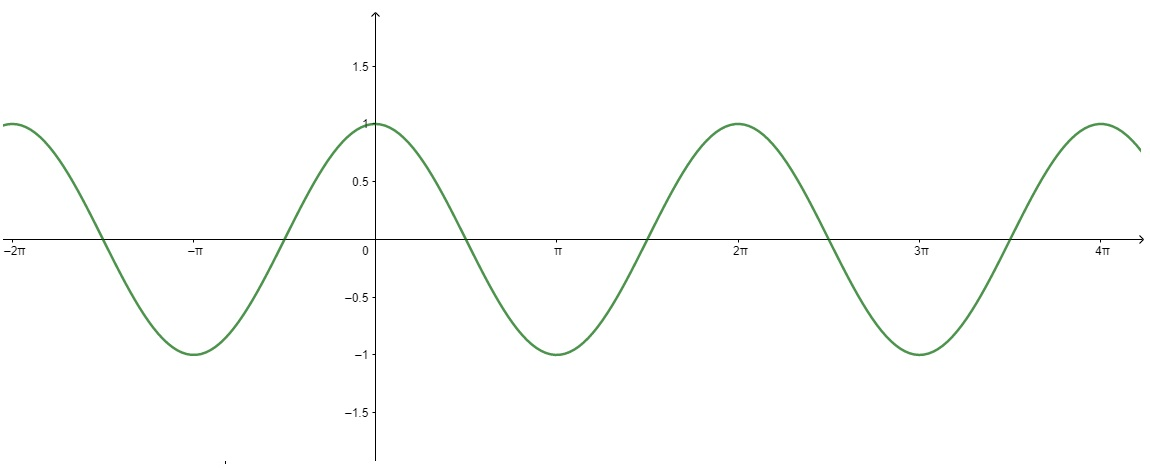
\includegraphics[scale=0.5]{\imgdirfromsection/grafcos.jpg}
\caption{Gráfico da função cosseno.}
\label{img:grafico-cosseno}
\end{figure}
\end{example}


\begin{example}
O gráfico da função $\sen: \reais \to \reais$ é mostrado na Imagem~\ref{img:grafico-seno}:
%
\begin{figure}[H]
\centering 
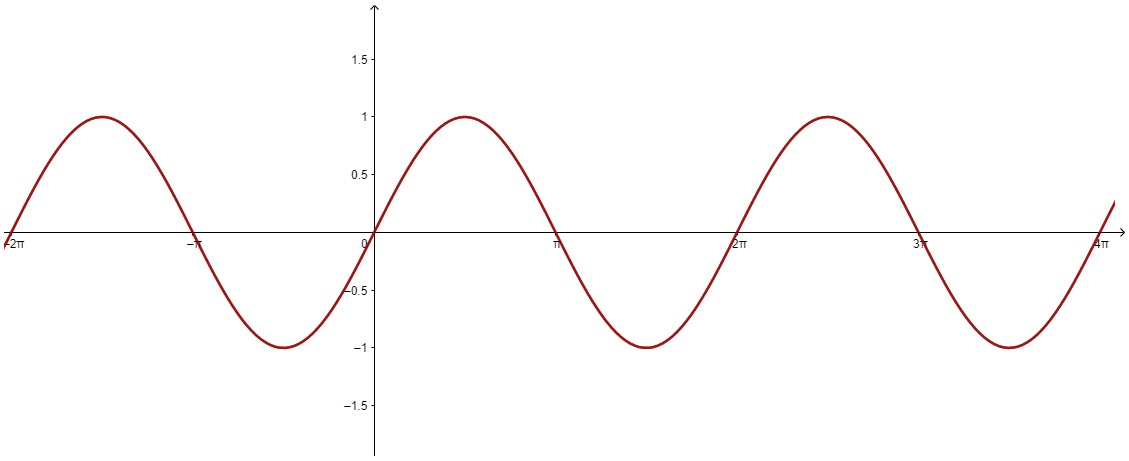
\includegraphics[scale=0.5]{\imgdirfromsection/grafsen.jpg}
\caption{Gráfico da função seno.}
\label{img:grafico-seno}
\end{figure}
\end{example}

\begin{onlineact}
    \khan{https://pt.khanacademy.org/math/trigonometry/trig-function-graphs/graphing-sinusoids/e/graphs_of_sine_and_cosine}
    {Gráfico de Funções Senoidais}.
\end{onlineact}